\documentclass[12pt, a4paper, twoside]{report}
\usepackage[utf8]{inputenc}
\usepackage{blindtext}
\usepackage[margin=2cm]{geometry}
\usepackage{markdown}
\usepackage[hyperref]{xcolor}
\usepackage{setspace}
\usepackage{newpxtext}
\usepackage{newpxmath}
\usepackage[margin=1cm, labelfont=bf]{caption}
\usepackage{subcaption}
\usepackage{booktabs}
\usepackage{numprint}
\usepackage{inconsolata}
\usepackage{mathtools}

\usepackage{graphicx}
\linespread{1.5}
\usepackage{xspace}
\usepackage{tikz-feynman}

% Biblatex
\usepackage[sorting=none]{biblatex}
\bibliography{bibliography}

% Hyperlinks
\definecolor{blue1}{RGB}{50, 142, 237}
\definecolor{red1}{RGB}{239, 83, 138}
\definecolor{orange1}{RGB}{243,109,33}
%\usepackage[colorlinks=true, allcolors=blue1]{hyperref}
\usepackage[colorlinks=true, allcolors=orange1]{hyperref}
\usepackage{soul}
\usepackage{amsmath}
\usepackage{bm}
\usepackage{marginnote}
\usepackage{adjustbox}

\usepackage{sepfootnotes}

%\usepackage[group-separator={,},separate-uncertainty=true]{siunitx}
\usepackage[separate-uncertainty=true]{siunitx}
\DeclareSIUnit\clight{\text{\ensuremath{c}}}


% Acronyms
\usepackage[acronym,nonumberlist]{glossaries}
\renewcommand*{\glstextformat}[1]{\textcolor{black}{#1}}
%\makeglossaries
\newacronym{COMET}{COMET}{Coherent Muon-to-Electron Conversion}

% Path of figures for each chapter
%\graphicspath{{introduction/}{chapter2/}{conclusion/}}

%
\newcommand{\diff}[2]{\frac{\textrm{d}{#1}}{\textrm{d}{#2}}}

% If table of contents goes too deep, we can limit depth.
%\setcounter{tocdepth}{0}

% Color scheme: 
%https://coolors.co/0081a7-00afb9-fdfcdc-fed9b7-f07167

\begin{document}

% % Title page
% \thispagestyle{empty}
% 
\includegraphics[width=0.4\textwidth]{IMP_ML_1CS_4CP.eps}
% \vfill
% \begin{center}
    
%     {\huge Thesis Title}
    
%     \rule{7cm}{1pt}
%     \vspace{2cm}
    
%     {\Large Matthias Dubouchet}
%     \vspace{1cm}
    
%     {\Large Department of High Energy Physics
    
%     Imperial College London}
%     \vspace{3cm}
    
%     {\large Submitted in partial fulfilment of the requirements\\for the degree of Doctor of Philosophy}
    
% \end{center}

% \vfill
% \clearpage

% % Blank page
% \shipout\null

% \pagenumbering{roman}

% \chapter*{Abstract}


COMET is a future high-precision experiment searching for charged lepton flavour
violation through the muon-to-electron conversion process. It aims to push the
intensity frontier of particle physics by coupling an intense muon beam with
cutting-edge detector technology. The first stage of the experiment, COMET
Phase\nobreakdash-I, is currently being assembled and will soon enter its data acquisition
period. It plans to achieve a single event sensitivity to $\mu$--$e$ conversion
in aluminium of $3.1 \times 10^{-15}$.

This thesis presents a study of the sensitivity and backgrounds of \mbox{COMET
Phase\nobreakdash-I} using the latest Monte Carlo simulation data produced. The background
contribution from cosmic ray-induced atmospheric muons is estimated using a
backward Monte Carlo approach, which allows computational resources to be
focused on the most critical signal-mimicking events.

Analysis of a $\mu$--$e$ conversion simulation sample suggests that COMET
Phase\nobreakdash-I will reach a single event sensitivity of $3.6 \times 10^{-15}$ within 146
days of data acquisition. In that period, the background contribution from
atmospheric muons is estimated to be 0.08 events under optimistic conditions,
namely a \SI{99.99}{\percent}-efficient Cosmic Ray Veto system and
\SI{99}{\percent} muon identification rate by the main detector.

% 
\chapter*{Declaration}
This dissertation is the result of my own work except where explicit reference
is made to the work of others. In addition, the methods and results reported in
Section~\ref{sec:quality_metrics} were investigated by a pair of MSci students
with my guidance.

\hfill Matthias Dubouchet

\vspace{2cm}
The copyright of this thesis rests with the author. Unless otherwise indicated, 
its contents are licensed under a Creative Commons Attribution-Non 
Commercial 4.0 International Licence (CC BY-NC). 
Under this licence, you may copy and redistribute the material in any medium 
or format. You may also create and distribute modified versions of the work. 
This is on the condition that: you credit the author and do not use it, or any 
derivative works, for a commercial purpose. 
When reusing or sharing this work, ensure you make the licence terms clear to 
others by naming the licence and linking to the licence text. Where a work has 
been adapted, you should indicate that the work has been changed and 
describe those changes. 
Please seek permission from the copyright holder for uses of this work that are 
not included in this licence or permitted under UK Copyright Law.

% \tableofcontents
% \printglossary[type=\acronymtype]
% \clearpage

% \pagenumbering{arabic}

\tableofcontents

\chapter{Backward Monte Carlo simulation for cosmic ray events}\label{ch:cosmics}

\begin{markdown}

1. Intro to BMC: relation to adjoint MC (find refs), maybe diagram

2. Physics: how we use BMC to determine rates of cosmic events: equations for
flux, sampling PDF, BMC weights, topography map of J-PARC

3. Integration into ICEDUST: implementation of sampling methods, event loop, output to
oaRooTracker format
+ `https://gitlab.in2p3.fr/comet/ICEDUST_packages/-/merge_requests/534`
+ `https://gitlab.in2p3.fr/comet/ICEDUST_packages/-/wikis/Backward-Monte-Carlo-sampling-with-SimBackwardMC#rate-calculation`

3. Actual estimation of background rate in Phase-I, maybe just quoting V's
result


\end{markdown}

% Intro: cosmics are important
Cosmic ray-induced events represent a significant part of the expected
background in the COMET experiment, as discussed in
Section~\ref{sec:backgrounds}. Cosmic muons irradiate the Earth at irregular
intervals and have a wide energy range, hence some fraction of them will be able
to mimic the conversion signal by entering the COMET detector system. 

Estimating the rate at which cosmic muons might produce signal-like events is
computationally expensive through standard Monte Carlo simulation methods. This
is due to the fact that the source of cosmic muons, i.e.\ the atmosphere, has a
much greater spatial extent than the active detector region. Hence, most cosmic
events generated from an atmospheric source will miss the detector completely
and not contribute in the estimation of the background rate, resulting in wasted
computation time.

A reverse (or adjoint) Monte Carlo simulation is one where the flow of particle
transport is reversed, i.e.\ events are generated in the sensitive detector
volume and propagated backward in time until they reach the source. This method
was initially used in 1967 to estimate gamma-ray and neutron radiation doses in
nuclear reactors~\cite{doi:10.13182/NSE68-A19235,doi:10.13182/NSE69-A19116}.
More recently, reverse MC has also been integrated into Geant4
simulations~\cite{DESORGHER2010247} for dosimetry in space, reversing the
electromagnetic physics of electrons, protons and ions.

In the case of muons, a backward transport method was developed by Niess et
al.~\cite{Niess_Barnoud_Carloganu_Menedeu_2018} in the context of muon
tomography, and it was later adapted to the COMET experiment in order to refine
estimations of the background rate from cosmic rays. This chapter discusses the
backward MC method for cosmic muons, how it is applied to COMET and the
resulting rate estimations in COMET Phase-I.


\section{Backward Monte Carlo transport}
In standard Monte Carlo simulations, events are generated by a source and
propagated forward in time according to their equations of motion and
interaction cross-sections within any surrounding medium. In a situation where
the source is large compared to the sensitive detector volume, as illustrated in
Figure~\ref{fig:bmc_configuration}, events have a high probability to miss the
detector and contribute nothing in the desired computation.

In backward MC, events are generated according to an arbitrary probability
density function (PDF) around the detector volume. The overall sampling PDF is
typically the composite of a position, direction and energy sampling
distributions, i.e.\ 
$$
p(\bm{x}, \bm{p}, E) = p(\bm{x}) \times p(\bm{p}) \times p(E),
$$
where $p$ denotes a PDF whose integral is 1, $\bm{x}$ denotes position, $\bm{p}$
direction and $E$ energy. 

\sepfootnotecontent{A}{See Reference~\cite{DESORGHER2010247} for a thorough
discussion of adjoint cross-sections, weights, weight corrections and source
normalisation.}

Each event is propagated backward using adjoint transport and interaction
kernels such that the probability of the event can eventually be determined. At
each step of the propagation, a multiplicative weight is computed from the
adjoint interaction cross-sections in the local medium. When the particle
reaches the source, the directional flux at the source is used as a
normalisation factor to yield the final event weight\sepfootnote{A}. Given a
significant enough sample of reverse events, the weights can be summed to
obtain the absolute flux or rate of particles hitting the detector.


% Interesting paragraph from desorgher:
%  The Monte Carlo sampling of a big enough number of reverse tracks is
%  equivalent to the integration of the weight W over all independent variable
%  (E1,O1,Sd,x1,E0, ...) summed over all type of reverse reactions, atomic
%  elements, adjoint primaries, and adjoint secondaries. In this integration the
%  cases where more than one reaction and no reaction occur are also considered
%  and only the tracks reaching the external source are accounted for. By this
%  way the same answer is obtained as in the forward case.

\begin{figure}
    \centering
    %\includegraphics[width=0.6\textwidth]{chapter5/qwe.png}
    \caption{BMC configuration.}
    \label{fig:bmc_configuration}
\end{figure}

% How does one estimate the rate of cosmics from the sampling PDF and BMC
% weights?
% Describe procedure / maths?

% We backward propagate the same event many times in order to get a reasonable
% rate estimate. Perhaps mention that.

\section{Cosmic muon rate estimation}
% Here, talk about the COMET setup: 
% + We want to estimate the rate of background events caused by 
%   muons+secondaries hitting the detector
% + Thus, we sample muons+/- around the envelope of the CRV, according to [spell
%   out PDF]
% + We apply backward MC up to an atmospheric muon flux model at altitude X,
%   tabulated from CORSIKA etc.
% + We can first estimate the cosmic muon rate on each surface of the CRV
%   Show plots etc.
% + From the events generated at the CRV envelope, it is also possible to
%   propagate forward to determine which events might produce signal-like
%   tracks.
% + Once this is done, we use the results from backward propagation to estimate
%   rate of background-inducing cosmic muons, qed.


% Do we talk about the PUMAS, GOUPIL setup?
% ICEDUST integration?

\chapter{COMET Phase-I sensitivity and backgrounds}

With the framework to simulate backgrounds from atmospheric muons in place, we
can now combine the results into a complete sensitivity and background
simulation study for COMET Phase-I. In this chapter, we discuss our simulation
samples consisting of signal, decay in orbit (DIO), and atmospheric events, and
present our resulting expectations of the performance of Phase-I.

\section{Simulation setup}
Three simulation samples are produced for this study. A $\mu$--$e$ conversion
sample, a DIO sample and an atmospheric muon sample. All three are simulated in
the geometrical world shown in Figure~\ref{fig:bmc_geometry}. This geometry
differs from the older TDR design~\cite{the_comet_collaboration_comet_2020} by
the number of counters in the CTH. Here, each layer of the CTH has 64 counters
instead of the original 48, which mainly affects the detector's geometrical
acceptance. In addition, the outer layer of the CTH is composed of plastic
scintillator counters rather than the Cherenkov counters, as was originally
planned. As we will see, this has an important effect on the detector's ability
to discriminate atmospheric anti-muons from conversion electrons.

\subsection{\texorpdfstring{$\mu$--$e$}{Muon to electron} conversion} 

\subsubsection{Sample}

The signal sample is the most straightforward to produce. We initially generate
primary electrons with energy $E=\SI{104.97}{\MeV}$ uniformly inside the
stopping target disks. Their direction is isotropically distributed, as would be
the case in the conversion process. A uniform position distribution in each disk
is not realistic, because the actual distribution depends on where in the
stopping target the muons in the beam become bound. To account for this, the
events are weighted according to the stopping positions of muons recorded in the
MC5 simulation. The weighting factor is determined from the relative probability
for a muon to stop at the sampled position, which is estimated by histogramming
the stopping positions in each disk.
Figure~\ref{fig:stopping_position_reweighting} shows the sampled uniform
position distribution and the resulting distribution after weighting. In total,
$N_\mathrm{signal} = 2\times 10^6$ events are simulated to compose the signal
sample.

% After applying geom cut of CTH trigger, how many remain?

\begin{figure}
    \centering
    \begin{subfigure}{0.46\textwidth}
        \centering
        \caption{Pre-weighting.}
    \end{subfigure}
    \hfill
    \begin{subfigure}{0.46\textwidth}
        \centering
        \caption{Post-weighting.}
    \end{subfigure}
    \caption{ Initial position distribution of signal electrons before and after
        weighting them by the likelihood of a muon being bound in each bin. }
    \label{fig:stopping_position_reweighting}
\end{figure}

\begin{figure}
    \centering
    
    \caption{Conversion signal event in the CyDet system.}
    \label{fig:signal_in_cydet}
\end{figure}

\subsubsection{Selection}
Signal events are selected based on detector acceptance criteria. We first require
fourfold coincidence in the CTH. The fraction of events remaining
defines the geometrical acceptance 
$$
A_\mathrm{geom} \equiv  \frac{\text{fourfold coincidences}}{N_\mathrm{signal}}.
$$
In our simulation setup with the 64-counters-per-layer CTH, our estimated
geometrical acceptance is $A_\mathrm{geom} = \SI{21}{\percent}$. In comparison,
the TDR cites $A_\mathrm{geom} = \SI{26}{\percent}$ with the previous design of
the CTH. 
\hl{Figure~X shows a conversion event which passes the
fourfold coincidence selection criterion.??}

% Reconstruction
We do not fully simulate the reconstruction of signal electron trajectories in
the CDC. In order to approximate the effect of reconstruction uncertainties, a
smearing is applied to the true momentum of each track. The reconstructed
momentum is estimated as $p_r = p_t + x$, where $p_t$ is the true momentum of
the electron as it enters the CDC, $x \sim \mathcal{N}(0, \sigma)$, and $\sigma
= \SI{200}{\keV/\clight}$ is the expected momentum resolution of the CDC.

% Other acceptance factors (not simulated)
Other acceptance criteria, such as the trigger timing window and reconstruction
quality cuts, are not properly simulated in this study. Instead, we apply
efficiency factors for each of them based on their TDR estimates.
\hl{Reference a table here?}


\subsection{Muon decay in orbit}
\subsubsection{Sample}
The DIO sample is similar to the signal sample in that the initial position
of signal and DIO electrons is identically distributed. Hence, we also sample
uniformly in the stopping target disks and then weight the events according to
the MC5 stopping position distribution. Similarly, the direction of DIO
electrons is sampled isotropically. The energy distribution is thus the only
difference between the two samples. 

\begin{figure}
    \centering
    
    \caption{Energy spectrum of DIO electrons from muonic aluminium atoms.}
    \label{fig:czarnecki_spectrum}
\end{figure}

The theoretical energy spectrum of DIO electrons produced in aluminium muonic
atoms was determined by Czarnecki et al.~\cite{czarnecki} and is shown in
Figure~\ref{fig:czarnecki_spectrum}. Their calculated spectrum is used to
determine an energy weighting factor for simulated DIO events. In a similar way
to the position weighting procedure, DIO events are first generated with a
uniform energy distribution, and then weighted according to the relative
likelihood for a DIO electron to have the sampled energy.
Figure~\ref{fig:dio_energy_reweighting} shows the weighted energy distribution
compared to the theoretical energy spectrum. \hl{FIGURE and then adjust text}.
The DIO sample is composed of $N_\mathrm{DIO} = 10^7$ events in total.

\begin{figure}
    \centering
    
    \caption{DIO-induced background with momentum  $p=\SI{1}{\MeV/\clight}$.}
    \label{fig:muon_dio_in_cydet}
\end{figure}

\subsubsection{Selection}
The selection of DIO events is identical to the selection of conversion events.
We require a fourfold coincidence in the CTH, and then apply a Gaussian smear to
the true momentum of the electron to simulate track reconstruction. The same
efficiency factors as for signal events are applied.

\subsection{Atmospheric muons}

\subsubsection{Sample}

Atmospheric muon events are simulated as explained in
Section~\ref{sec:cosmic_event_sampling}. Two samples are produced, one on the
entire surface of the CRV and one more densely concentrated on its upstream and
downstream openings. Because of how rarely a sampled atmospheric event produces
signal-like features, the atmospheric dataset is by far the largest of the
three, with $1 \times 10^9$ events generated on the envelope and $1.4 \times
10^9$ on the openings.



\begin{figure}
    \centering
    
    \caption{Cosmic ray-induced background with momentum $p=\SI{1}{\MeV/\clight}$.}
    \label{fig:cosmic_bg_in_cydet}
\end{figure}


\hl{TODO remove below}

The time distribution of signal, DIO and atmospheric events is not realistically
simulated in this study. Instead, we apply an average timing window efficiency
factor to all events in order to estimate the total count integrated over
data-acquisition time.

The time efficiency factor is not the same for signal, DIO and cosmics,
because they don't have the same time distribution. For cosmics, the time
distribution is ~uniform, so the factor should just be live time / (live +
dead time). For signal and DIO, it is dependent upon the time distribution of
muon bound in the tgt.

\subsubsection{Selection}
\hl{TODO}


\subsection{Sample weighting}
\sepfootnotecontent{fn:conv_br_norm}{The nuclear muon capture branching ratio appears in this
expression because the branching ratio of $\mu$--$e$ conversion is
conventionally normalised to $\mathcal{B}_\mathrm{capture}$.}

Because they originate from different processes, the three MC samples must be
weighted differently in order to determine the absolute contribution from each.
The conversion and DIO processes both originate from the muons bound in the
stopping target, hence we can express the total number of expected conversion
and DIO electrons in terms of the total number of stopped muons $N_\mu$.
The number of signal electrons, as a function of the conversion branching
ratio $\mathcal{B}_\mathrm{conversion}$, is:
$$
N_{e^-}^\mathrm{conversion} = 
N_\mu \, \mathcal{B}_\mathrm{conversion} \, 
\mathcal{B}_\mathrm{capture} \, f_\mathrm{coherent},
$$
where $\mathcal{B}_\mathrm{capture} = 0.61$ is the branching ratio of nuclear
muon capture\sepfootnote{fn:conv_br_norm} and $f_\mathrm{coherent}=0.9$ is the
fraction of conversions that are coherent. Similarly, the total number of DIO
electrons can be expressed as:
$$
N_{e^-}^\mathrm{DIO} = N_\mu \, \mathcal{B}_\mathrm{DIO},
$$
where $\mathcal{B}_\mathrm{DIO} = 1 - \mathcal{B}_\mathrm{capture} -
\mathcal{B}_\mathrm{conversion} \approx 0.39$ is the branching ratio of DIO.


In the case of atmospheric muons, the backward MC procedure yields an absolute
rate. This rate is multiplied by the total data acquisition (DAQ) time of the
experiment to obtain the expected background count:
$$
N_\mathrm{atmospheric} = R \times T_\mathrm{DAQ},
$$
where $R$ is the total atmospheric background rate, and we set
$T_\mathrm{DAQ}=146$ days, corresponding to $N_\mu = 1.5\times 10^{19}$, in this
study. 

\subsubsection{Trigger time window efficiencies}
In order to take into account the trigger timing window, we assume that
atmospheric muons irradiate the detector with a uniform time distribution.
Hence, the time window efficiency factor is simply the average fraction of
time when the trigger is active:
$$
\epsilon_\text{time window}^\mathrm{atmospheric} =
\frac{8}{9}\,\frac{1170 - 700}{1170} = \SI{36}{\percent}
$$
assuming the trigger window is between 700 and \SI{1170}{\ns}, and where the
factor $\frac{8}{9}$ arises from the bunch structure of the J-PARC main ring. In
contrast, the efficiency factor for conversion and DIO electrons
$\epsilon_\text{time window}^\text{conversion|DIO} \approx \SI{30}{\percent}$ is
smaller because the time distribution of bound muons peaks around \SI{300}{\ns},
before the trigger becomes active (see Figure~\ref{fig:timing_distributions}).



\section{Single event sensitivity}
The single event sensitivity (SES) is defined as the value of the $\mu$--$e$
conversion branching ratio required for the experiment to observe one signal
event. It can be expressed in terms of the experimental acceptance $A_{\mu-e}$ and the
total number of muons stopped in the stopping target $N_\mu$:
\begin{equation}
    \mathrm{SES} = \frac{1}{N_\mu\,A_{\mu-e}\,\mathcal{B}_\mathrm{capture}\,f_\mathrm{coherent}},
\end{equation}
where $\mathcal{B}_\mathrm{capture} = 0.61$ is the branching ratio of nuclear
muon capture and $f_\mathrm{coherent} = 0.9$ is the fraction of conversions
expected to leave the nucleus in its ground state.

% Is it worth ELI5 here?
% The net signal acceptance $A_{\mu-e}$ is the product of various factors stemming
% from the experiment's design and inefficiencies in the processing,
% reconstruction and selection of candidate events. 

% How do we approach the fact that CTH geom has changed so our geom acceptance
% is lower?

\hl{ v We've already mentioned trigger selection and acceptance in the Selection
    subsec of every sample. Cut.}
    
In this study, the CTH trigger mechanism was simulated by finding events
involving a fourfold coincidence. The fraction of signal events which induce a
trigger is defined as the geometrical acceptance $A_\mathrm{geom}$. In our
simulation setup, the CTH contains 64 counters per layer, two layers
in each module, one module at the upstream end of the CDC and the other
downstream (256 counters in total). Our estimated geometrical acceptance is
$$
A_\mathrm{geom} \equiv \frac{\text{fourfold coincidences}}{N_\mathrm{signal}} = \SI{21}{\percent}.
$$
In comparison, the COMET Phase-I TDR~\cite{the_comet_collaboration_comet_2020}
cites $A_\mathrm{geom} = \SI{26}{\percent}$ with the previous design of the CTH,
which had 48 counters per layer. This reduced acceptance worsens the sensitivity
of the experiment slightly. In this study, none of the other experimental
aspects that contribute to the net acceptance were changed, hence we use the
other factors of $A_{\mu-e}$ from the TDR, and only replace the value of
$A_\mathrm{geom}$ with the newly estimated one. Values of the acceptance
coefficients used in our study are shown in Table~\ref{tab:acceptance}. The net
signal acceptance using these factors is $A_{\mu-e} = 0.032$.

The number of muons stopped in the stopping target, $N_\mu$, is a function of
the COMET beam power, the target material, the design of the
transport system, and the total data-acquisition time. 
The target material sets the yield of
backward-going pions which will decay to muons of the right momentum to come at
rest in the muon stopping target. This, combined with the transport system,
determines the yield of stopped muons per proton collision $R_{\mu/p} \equiv
\frac{\text{muons stopped}}{\text{proton on target}}$. Here, we use the
MC5 dataset, a sample of $10^9$ POT collisions, to estimate $R_{\mu/p}=4.86
\times 10^{-4}$.
The beam power and data-acquisition time together determine the total number of proton
collisions that will occur. COMET Phase-I requires $N_\mathrm{POT} = 3.15 \times
10^{19}$ collisions in order to reach its sensitivity goal, corresponding to a
data-acquisition time of $T=146$ days.
These figures allow us to estimate the total number of stopped muons
$$N_\mu = R_{\mu/p} \times N_\mathrm{POT} = 1.56\times 10^{16},$$
which can be substituted into the SES formula:
\begin{equation}\label{eq:my_ses}
\mathrm{SES}
=\frac{1}{N_\mu\,A_{\mu-e}\,\mathcal{B}_\mathrm{capture}\,f_\mathrm{coherent}}
= 3.81\times10^{-15}.
\end{equation}
This value is slightly worse than the TDR estimation,
$\mathrm{SES}_\mathrm{TDR}=3\times 10^{-15}$, because of our lower geometrical
acceptance when using the new CTH design.

% \begin{table}
%     \centering\begin{tabular}{l|ccc}
%         \toprule
%         a&b&c&d\\\midrule
%         a&b&c&d\\
%         \bottomrule
%     \end{tabular}
%     \caption{ Acceptance coefficients used to estimate the single event
%     sensitivity in Equation~\ref{eq:my_ses}. These also apply to the
%     decay-in-orbit background rate estimation. }
%     \label{tab:ses_efficiency_factors}
% \end{table}


\section{Momentum spectra}
Because the signal has a clear mono-energetic signature, a precise measurement
of the momentum of candidate tracks helps to discriminate signal from
backgrounds. Figure~\ref{fig:log_spectrum} shows the momentum spectrum
for candidate conversion, DIO and atmospheric events.

\begin{figure}
    \centering
    
    \caption{Log spectrum.}
    \label{fig:log_spectrum}
\end{figure}

\section{Discussion}

\subsection{Atmospheric $\mu^+$ backgrounds}

\subsection{CRV efficiency}

\subsection{Particle identification}

\appendix
\chapter{Integration of backward Monte Carlo software into
ICEDUST}
\label{app:bmc_integration}

% \begin{itemize}
%     \item External packages: PUMAS, GOUPIL, GOUPIL components. Cite~\cite{NIESS2022108438}.
%     \item Internal package: SimBackwardMC
% \end{itemize}


\section{Original implementation}
The backward Monte Carlo simulation software was originally written and applied
to the COMET Phase\nobreakdash-I experiment by Valentin Niess, author
of~\cite{Niess_Barnoud_Carloganu_Menedeu_2018,NIESS2022108438}.
Figure~\ref{fig:pumas_integration_strategy} shows the layout of the original set
of software layers used to run backward MC simulations in the Phase\nobreakdash-I world. 

At the core of the backward Monte Carlo simulation is the backward transport
engine, PUMAS~\cite{NIESS2022108438}. PUMAS is responsible for the propagation
of particles through matter and the computation of MC weights based on the path
taken and the interactions undergone, as discussed in
Section~\ref{sec:bmc_method}. Because it is designed exclusively for this
purpose, PUMAS does not provide utilities for navigating through complex
geometries or sampling the flux from pre-computed tables. Another package,
GOUPIL, takes on this role as an interface to PUMAS, and allows the user to
specify a geometry, a source flux, as well as the local topography and
geomagnetic field around the experiment's location. An additional interface
between GOUPIL and {\sc Geant4}, \texttt{goupil-geant4}, was developed to allow
the user to control backward MC runs with the {\sc Geant4} macro user interface
and to load and navigate the geometry from a GDML file. The final layer,
\texttt{resample-simg4}, provides a command-line interface and enables events
generated by \texttt{SimG4} to be read as input for the backward MC simulation
to estimate their flux.


\begin{figure}
    \centering
    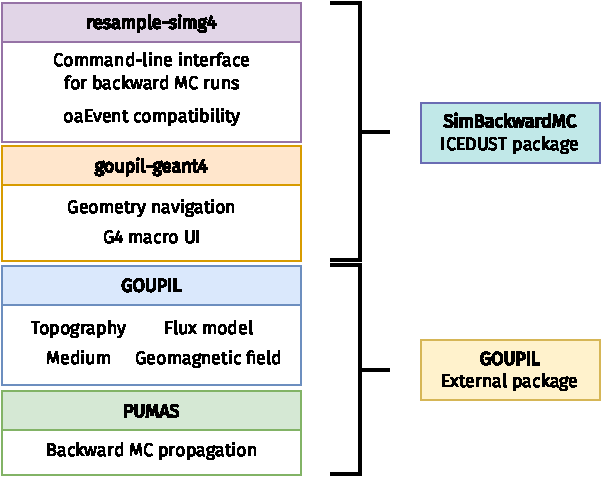
\includegraphics[width=0.6\textwidth]{appendixA/integration_strategy.drawio.pdf}
    \caption{ Software packages that compose the original backward MC simulation
        stack for the Phase\nobreakdash-I study, and organisation of their integrated
        ICEDUST counterparts.}
    \label{fig:pumas_integration_strategy}
\end{figure}

\section{Integration}

Figure~\ref{fig:pumas_integration_strategy} also shows how the original software
was arranged to become part of the ICEDUST framework. Since the PUMAS and GOUPIL
packages are unlikely to undergo quick iterative changes over time, they are integrated
into an external package. The functionalities of the upper two layers of the
stack are combined into a new ICEDUST package called \texttt{SimBackwardMC}.

The way in which the layers are organised is not the only difference between the
original and current software. Three major changes were implemented during the
integration in order to bring the original software closer to the ICEDUST
workflow.

\begin{itemize}
    \item {\bfseries Geometry format:} originally read from GDML files, the
    geometry is now created from the same classes and macro files that define
    the simulation world in forward MC runs by the \texttt{SimG4} package. This
    additionally ensures that the geometry used in forward and backward MC
    simulations is identical.
    \item {\bfseries Entry point:} the main \texttt{resample-simg4} entry point
    was previously a Lua script executed via LuaJIT which defined the
    command-line interface, configured the backward simulation run, and
    processed the output. \texttt{SimBackwardMC} uses a standard ICEDUST event
    loop executable as its entry point to handle command-line arguments, read
    events from input \texttt{oaEvent} files and output the results of the
    backward simulation.
    \item {\bfseries Output format:} \texttt{resample-simg4} wrote the results
    of backward sampling to a text file in a format similar to CSV.
    \texttt{SimBackwardMC} writes to a \texttt{RooTracker} file instead, since
    that is a standard ICEDUST format and a good fit to store the kinematics of
    processed events along with their estimated flux.
\end{itemize}

The integrated backward MC software presented here was used to obtain the
results of Chapters~\ref{ch:cosmics} and~\ref{ch:phase-I_study}. It is also
currently being used in the work of others, for instance to estimate the
atmospheric muon flux at various locations around the Phase\nobreakdash-I detector system
and validate the results with real measurements. Through our standardisation of
some parts of the original software and the addition of specific documentation,
we hope that the \texttt{SimBackwardMC} package will remain a readily accessible
tool for future cosmic ray studies in COMET.


\printbibliography

% \listoffigures
% \listoftables

\end{document}
